\chapter{Review of Concepts}
\label{chapter-review}

\begin{abstract}
    The purpose of this chapter is to provide background knowledge and definitions of key concepts that are essential when addressing the identified research question. First, the concept of deep uncertainty is codified in \cref{review-uncertainty}. \cref{review-robustness} investigates recognized definitions of robustness in literature. Then, \cref{review-methods} explores the foundations and key concepts for each of the selected robust decision support methods. Finally, the stylized policy problem identified in the research definition is discussed in \cref{review-problems}, along with the relevant policy implementation structures.
\end{abstract}

\newpage

\section{Deep Uncertainty}\label{review-uncertainty}
Uncertainty is generally defined as the state of something not being known or not being completely certain \citep{def:uncertain}. Uncertainty due to a lack of information, even despite growing scientific knowledge has long been discussed in philosophy and scientific research \citep{Tannert892}. Modern research into the concept began with Frank Knight, who was one of the first to distinguish types of uncertainty: knowable uncertainty or Knightian risk, which can be converted easily into effective certainty through probabilities or other means, and true uncertainty or Knightian uncertainty, which cannot be measured or described effectively \citep{Knight1921}. Similarly, Edward Quade developed two categories of uncertainty: stochastic and real. Stochastic uncertainty is similar to Knightian risk and can be quantified using probabilities, while real uncertainty is similar to Knightian uncertainty and is the result of unknowable futures or actions \citep{Quade1989}. Knightian or real uncertainty provides the foundation for a concept called deep uncertainty. The formal definition of deep uncertainty that has become commonly accepted in policy analysis research was developed by \citet{Lempert2003}: 

\begin{conceptbox}\label{def:deepuncertainty}
    Deep uncertainty exists in policy problems when analysts do not know or cannot agree on one or more of the following three elements:
    \newline
    \begin{enumerate}[leftmargin=*]
        \item The model(s) that correctly describe relationships between key system elements that will shape the future
        \item The probability distributions that best represent uncertainties in key system elements
        \item The manner in which to rank the desirability of potential outcomes
    \end{enumerate}
\end{conceptbox}

Given the nature of wicked policy problems as established in \cref{chapter-intro}, deep uncertainty is an unavoidable obstacle to the decision support process. Whereas traditional policy analysis focuses on using a predict-then-act model to find the optimal solution, the presence of deep uncertainty means that accurate prediction and determination of what an optimal solution is become extremely difficult, if not impossible. When the focus for problems with deep uncertainty is on the search for an optimal solution, assumptions must be made in several areas: 

\begin{itemize}
    \item To determine all possible future scenarios and of their likelihood
    \item To define the probabilities and value ranges that describe identified uncertain variables
    \item To understand and operationalize what criteria an optimal solution must meet. 
\end{itemize}

Each of the elements required for optimal search, therefore, directly contravene the properties of deeply uncertain problems defined here. Because the correctness of a model that describes potential futures cannot be agreed upon, there is no way to concretely determine future scenarios and their likelihood. And continuing to the second point, the presence of deep uncertainty means that is no agreement on specification of uncertainties and their quantitative values. So, there can be no certainty about the values of identified sources of uncertainty. And finally, because there is a lack of agreement on what makes a potential solution more desirable than another, there can be no concrete definition of what makes a solution optimal. Instead, policy making must focus on a different evaluation method that looks to satisfy stated goals instead of optimize the system at hand. 

\section{Robustness}\label{review-robustness}
As the search for an optimal solution is recognized as an impossible task when faced with deeply uncertain problems, policy makers have instead looked to an alternate mechanism to analyze the goodness of potential solutions: robustness \citep{Maier2016}. The concept of robustness has a long history in engineering, economics, supply chain management, and many other fields \citep{Capano2017, Maier2016}. Engineering considers a robust system as one who is able to maintain functionality in the presence of failure of a part of the system \citep{Capano2017}. In biological robustness is seen as the ability for a system to maintain development despite external perturbations \citep{Jen2003}. Robustness of organizations is viewed as the ability of that organization to maintain its function through changing internal and external conditions \citep{Capano2017}. Common among these definitions is that robustness of a system of any type exists when that system is able to maintain core functionality in the face of external change. This concept of robustness will be used as the foundation for robustness in policy analysis. 

Robustness in policy analysis can be defined in multiple ways. First, it is possible to define robustness at a system level, where the system is most often represented as a model that describes the uncertainties, policy levers, relationships, and desired outcomes that is used to analyze the problem of interest. Robustness of a system can be defined similarly to robustness of natural systems. A robust system has the ability to maintain its functions despite changes in internal or external factors \citep{Capano2017}. Defined in this way, robustness becomes distinct from other possible measures of system performance: resilience, stability, and adaptability. A robust system is able to maintain functionality but is not required to maintain the same state, where a resilient or stable system is able to maintain the same state. And in contrast to robustness, adaptability can be considered a property of a lever or policy that helps a system maintain robustness \citep{Capano2017}. 

Robustness can also be defined for a policy, which is generally represented as a set of possible lever values. This definition of robustness will be the focus of this research. The following is a general definition of robustness as defined for potential policies of a specific system: 

\begin{conceptbox}\label{def:robustness}
    A robust policy is one that performs well across a variety of possible future states of a system, due to both internal and external changes \citep{Herman2015,Kasprzyk2013,Matrosov2013a,WalkerLempertKwakkel2013}. 
\end{conceptbox}

Instead of searching for the optimum solution, by seeking a set of solutions based on robustness, the search process will better avoid finding solutions that are overly sensitive to changes in uncertain parameter values. It is possible for the optimum solution of a system to belong to the set of solutions that are considered robust (which is known as a super-robust solution). However, it is much more common that the robust solution to have lower performance than the optimum solution given a set of uncertain parameter and decision lever values \citep{Sniedovich2016}. This is known as \textit{the price of robustness} \citep{Bertsimas2004}. 

Robustness of a policy can be analyzed from multiple perspectives: resistance to change, avoidance of change, recovery from change and adaptability in response to change \citep{Durach2015,DeGoede2013,Twomey2012}. Because there are several facets to a policy's robustness, there exists many established robustness metrics, each prioritizing a different facet of robustness. Calculation of each of these metrics generally involve the same three elements: determination of the different decisions that could be made, outcomes of interest or performance metrics, and the scenarios or possible future states of the world that will be considered. Robustness metrics may determine performance as an absolute calculation or relatively to other policies. Each metric also employs differing levels of risk aversion: include more extreme scenarios in calculations to have a higher level of risk aversion. Finally, each metric has a different method of combining robustness calculations across scenarios for a specific policy option, including mean, standard deviation, skewness, or kurtosis \citep{McPhail2018}.

The following are a selection of robustness metrics that have been identified in previous policy and system analysis literature. The first group of methods listed below can be considered classical robustness metrics who use the absolute value of a performance measure to determine robustness, and report a robustness value with the same units as the performance measure under consideration \citep{McPhail2018}. The benefit of methods that directly communicate system performance mean that it is extremely simple to communicate the elements that make a policy alternative robust. 

\textbf{Minimax (strict robustness):} a worst-case approach that seeks the best performance under the worst case analyzed. Worst case scenarios are often black swan types of event \citep{Taleb2007}, where a black swan event is one that is rare, unexpected, and has a significant impact on a system. Because black swan events are inherently rare, they do not represent a good estimate of actual performance. Minimax is therefore an extremely conservative approach to determining robustness of a policy. The value of such a conservative approach depends on the problem under consideration. If costs of a worst case scenario are extremely high, then it makes sense to consider that worst case scenario in robustness calculations. However, under many other conditions, a worst-case scenario does not lead to catastrophically high costs, so determining a policy's robustness based on performance under the worst-case scenario may lead to unnecessarily expensive or conservative solutions. 

\textbf{Maximax:} follows a similar principle as the minimax criterion, but focuses instead on best case performance instead of worst case \cite{McPhail2018, Rosenhead1972}. By focusing the extreme positive range of values for an outcome, the maximax metric may ignore catastrophic conditions in the worst case scenario, leading to significant negative problems for decision makers. 

\textbf{Hurwicz optimism-pessimism rule:} representing the middle ground between minimax and maximax, Hurwicz rule involves a weighted average between the two metrics, with the weighting up to the decision maker to determine robustness \citep{Rosenhead1972}. Because the weighting is left up to decision makers, they are able to customize this metric according to their desired level of risk aversion \citep{McPhail2018}. 

\textbf{Laplace's principle of insufficient reason:} by assigning equal weight to all possible scenarios, robustness is determined as the mean of all values for an outcome \citep{Rosenhead1972}. This results in a robustness metric that has an average level of risk aversion. 

Other methods in this category include maximin, percentile-based skewness and peakedness, and mean-variance. 

The methods listed next calculate robustness based on relative performance, but produce outputs with the same units as the considered performance metric, making communication of robustness with decision makers a straightforward process. In this case, the robust option is one in which minimizes the maximum regret \citep{McPhail2018}

\textbf{Minimax Regret and 90th percentile minimax regret:} seeks to minimize regret with respect to the worst-case performance (or the 90th percentile of the worst case). Similar to the minimax metric, these metrics are conservative and have high risk avoidance.

\textbf{Undesirable deviations:} unlike minimax regret, this metric determines robustness as the deviation of the mean of the lower 50th percent of performance values from th median performance, given the set of performance measures over an ensemble of scenarios \citep{Kwakkel2016Robust}. This method results in a level of risk aversion that is lower than that found in minimax regret and 90th percentile regret, but still maintains a relatively high level of risk aversion \citep{McPhail2018}

Instead of determining robustness that indicate actual system performance, the final robustness calculation considered here indicates only whether the system is performing satisfactorily or not. Satisficing metrics use the value of performance measures directly, but will report a relative robustness value that indicates whether performance is satisfactory \citep{McPhail2018}. There are many satisficing metrics available, the most common of which is described below: 

\textbf{Starr's domain criterion:} defines robustness based on the number of scenarios in which a performance measure meets a decision maker's defined threshold \citep{Hadka2015}. Because the threshold for performance is determined by the decision maker, she is able to customize this metric according to her preferred level of risk aversion.

Common among these metrics is that each is defined with respect to some value or set of conditions that must be established based on the problem that is being analyzed. Therefore, a policy's robustness value is only valid under conditions specific to the system being analyzed and to the definition of robustness used. At the same time, selection of the appropriate metric to use is based primarily on decision maker objectives, but may also depend on limitations of the method that is used for analysis. Combining the wide variety of possible robustness metrics, each of which measure robustness in a different manner, the subjectivity of metric selection, and the fact that robustness values are only valid in the specific problem and analysis context under which they are calculated, it becomes difficult to asses the real-world robustness of a system, given a specific policy implementation. 

Several studies have been completed that compare different robustness metrics given a specific problem \citep{Giuliani2016, Herman2015, Kwakkel2016Robust, Roach2016}. These studies have generally concluded that each robustness metric indicates a different facet of the robustness of a potential policy. This makes it difficult to compare robustness across different metrics and can lead to confusion between decision makers, who must determine how to use the analysis and robustness values in their decision-making process. \citet{McPhail2018} propose a framework that categorizes the different robustness metrics based on several factors, including required inputs, method of calculation, unit of output, and level of risk aversion. This taxonomy aims to assist decision makers in determining the most appropriate metric to use when analyzing their own problems. And while this guidance may provide a stronger foundation with which to select a specific robustness metric, selection of a specific metric will still have a significant impact on the policy recommendation process. 

Given that it is impossible to identify a single optimum policy in the case of a deeply uncertain problem and armed with the knowledge required to define a policy's robustness instead of it's  absolute performance, a prescriptive method to determine policy alternatives and their robustness is required.

\section{Robust Decision Support Methods}\label{review-methods}
The search for robust solutions instead of the optimal one requires assessment of  different potential solutions over a large ensemble of possible future states of the world, also known as scenarios. Exploratory Modeling and Analysis (EMA), is a technique that can be used as a foundation for methods that support this process. This technique advocates the use of computational experiments that describe the range of potential future states of the world of a system and to use those experiments to explore the behavior of that system in response to different policy settings \citep{Bankes1993}. EMA techniques have integrated into the robust decision support methodology, which is descried next. 

    \subsection{Robust decision making}\label{review-rdm}
    Analysis of deeply uncertain wicked problems brings along with it several requirements. First, that policies should be analyzed with respect to robustness and not optimality (which was discussed in \cref{review-robustness}). Second, that the set of potential futures cannot be represented as a small number of possibilities (given the large amount of uncertainty that is frequently influenced by multiple input variables, it is generally impossible to codify a short list of possible futures for a problem), but has to instead be described using large ensembles of potential futures, with the number of scenarios stretching anywhere from a few hundred to several million. Analysis of these problems must also lead to results that can be clearly communicated to decision makers, to ensure that any conclusions are not just used to inform decisions, but are interpreted correctly. Furthermore, wicked problems characterized by deep uncertainty commonly involve multiple decision makers and always include conflicting views on model and input specification, and on output ranking. Because of these factors, any decision making process must be iterative, providing the opportunity for feedback from decision makers and model or policy refinement based on that feedback \citep{Tsoukias2008}. 
    
    \citet{Lempert2003} proposes a prescriptive and systematic method to support decision making of problems with characteristics similar to a wicked problem known as robust decision making (RDM) that attempts to address many of the factors listed above. The proposed method involves an iterative process of model and policy specification, computer aided computational experimentation that involves the generation and execution of a large ensemble of scenarios that span the defined uncertainty space, development of interactive visualizations, and decision maker input and refinement based on the results of computational experimentation and generated visualization \citep{Lempert2006}. For the purposes of this research, a description of the method flow can be found as \cref{fig:rdm-flow}. 

    \begin{figure}[ht]
        \centering
        \captionsetup{justification=centering}
        
        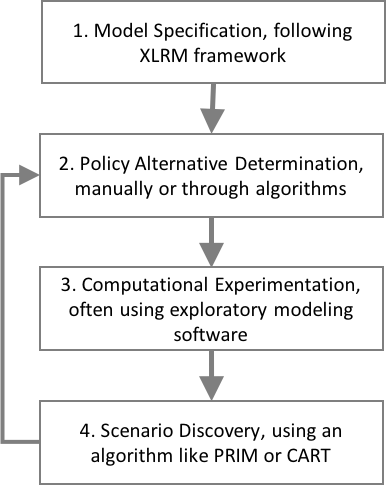
\includegraphics{rdm-flow}
        \caption{Robust Decision Making Process}
        \label{fig:rdm-flow}
    \end{figure}
    
    The first step of any formal analysis must be to organize any relevant information into a usable form. In the case of RDM, this step is referred to as model specification. To accomplish this, \citet{Lempert2003} proposes a 4-category structure with which to organize model elements, known as the XLRM framework. "X" refers to the exogenous uncertainties that are outside of the control of decision makers but still impact behavior of the system being considered. Variables that are controlled by decision makers are categorized under "L", also known as policy levers. The desired outcomes of interest are categorized as measures, or "M". Finally, relations ("R") describe how each of the elements in the "X", "L", and "M" categories relate to one another. Together, the items described by each of the 4 categories become the model that will be used for the remainder of analysis.

    \begin{figure}[ht]
        \centering
        \captionsetup{justification=centering}
        
        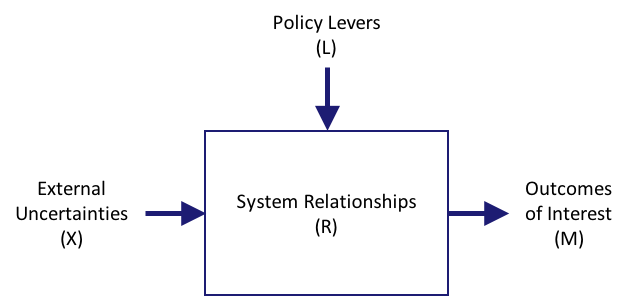
\includegraphics{xlrm}
        \caption{The XLRM Framework \citep{Kwakkel2017}}
        \label{fig:xlrm}
    \end{figure}
    
    As a part of the structuring of data and information, the second step of the RDM process involves identifying policy alternatives, also known as candidate strategies. The selection process can manifest in many different ways. Decision makers may contribute a set of initial strategies that will be considered \citep{Lempert2006}. Alternatively, analysis can leverage the specified model to determine policies based on sensitivities to identified sources of uncertainty or decision levers through a traditional sensitivity analysis.
    
    In step three, the XLRM specification is used to build a diverse ensemble of possible future states of the world (SOWs), or scenarios, that span the uncertainty space specified in the first step. The set of future SOWs are used to determine how the defined policies may react to a wide variety of possible futures. This stage generally involves the use of software to both build the ensemble of scenarios and to apply that ensemble to the set of policy options to build a data set that evaluates the potential effectiveness of a policy given the XLRM problem definition. 

    Once the evaluation data is built through computational experimentation in step 3, that information is used to calculate policy robustness and to discover vulnerabilities in the existing policy options based on the identified robustness measure (possible robustness metrics were discussed in \cref{review-robustness}, but RDM traditionally favors a satisficing measure \citep{Matrosov2013b}). The process of searching for vulnerabilities is known as Scenario Discovery. PRIM (the Patient Rule Induction Method) is typically identified as the most suitable scenario discovery method for RDM, as it produces simple rules that accurately determine the factors (both uncertainties and policy settings) which contribute to poor performance \citep{Lempert2006}. This information is used to refine both the model and policy options in an iterative process until the analyst and other decision makers reach a policy option or set of options that they can implement to address the problem. 
    
    Together, these four steps formed an iterative process that is one of the first attempts to develop a prescriptive method to guide the decision making process under conditions of deep uncertainty. The RDM method as it stands falls short in one key way. First, when there is deep uncertainty present in an analysis, there are going to be many decision makers involved who don't agree on the proper XLRM specification and who will have conflicting objectives \citep{WalkerLempertKwakkel2013}. Though the RDM process does support decision maker interaction throughout the process, it does not codify a formal mechanism for determining different policy options when faced with conflicting objectives \citep{Kasprzyk2013}. Other methods of decision support have been developed that build on the RDM structure but seek to address this shortcoming, which will be reviewed next. 

    \subsection{Multi-objective robust decision making (MORDM)}\label{review-multi}
    Building on the foundation of RDM, \citet{Kasprzyk2013} propose a decision support method called multi-objective robust decision making (MORDM), which provides a structure for managing a wide spectrum of decision maker perspectives and conflicting objectives. \cref{fig:mordm-flow} indicates how MORDM has been adapted from RDM. The most significant change is the introduction of a formal process to determine potential policy alternatives in step 2 through the application of a multi-objective evolutionary algorithm (MOEA). The MOEA searches for potential policy solutions and ranks them based on performance of the system at a base reference point (which is determined with decision maker input). A policy alternative is added to the Pareto non-dominated set of alternatives if its performance in the base reference scenario is not outperformed by another member of that set. By leveraging an MOEA, the MORDM process is able to quantify outcomes of interest that represent conflicting objectives and account for the conflict directly in this search phase. 
    
    \begin{figure}[ht]
        \centering
        \captionsetup{justification=centering}
        
        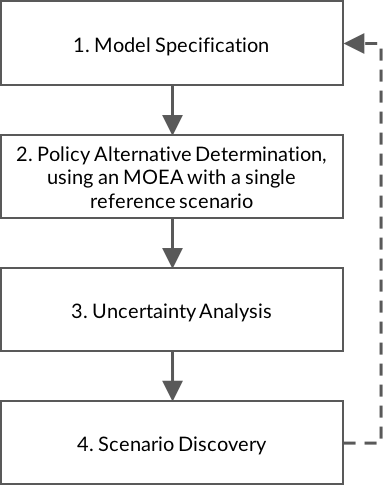
\includegraphics{mordm-flow}
        \caption{Multi Objective Robust Decision Making Process}
        \label{fig:mordm-flow}
    \end{figure}

    The MORDM method also codifies the process with which to help select a preferred solution from the set of solution alternatives generated with the MOEA, through uncertainty analysis, scenario discovery, and interactive visualizations \citep{Kasprzyk2013}. After model specification and an MOEA search for policy alternatives, the performance of the list of alternatives is tested under the recognized deep uncertainties through a process known as uncertainty analysis. This involves building a set of alternative future states of the world by sampling across the set of uncertainty parameters, a specified sampling method. Though there are many techniques available, from Monte Carlo to full and partial factorial, \citet{Kasprzyk2013} recommends using Latin Hypercube Sampling, which ensures that each member of the uncertainty set is represented evenly across the sampled set of SOWs \citep{Mckay1979}. 
    
    The data gathered from exercising each alternative policy over the set of SOWs provides the required information to perform a robustness analysis, in which a robustness metric is selected in a similar manner to the RDM method and robustness of each policy is calculated on a per-objective basis. This information is communicated through interactive visualizations that decision makers can leverage examine the robustness of policy alternatives and to better understand the trade-offs that exist between conflicting objectives. At this point, candidate strategies are selected by the decision maker for further analysis, through the scenario discovery process. Scenario discovery in the MORDM method is similar to that in the RDM method, where candidate policy alternatives are tested to determine potential vulnerabilities \citep{Bryant2010}. The MORDM method also supports an iterative structure wherein the information gathered in the uncertainty analysis and scenario discovery process can be used to refine potential policy alternatives. However, as MORDM leverages an MOEA to determine alternatives, any refinements occur at the model specification level, where new information can be used to adjust the uncertainty space or to influence the set of available decision levers, instead of the policy alternative determination phase (see \cref{fig:rdm-flow} and \cref{fig:mordm-flow}). 
    
    Because of the changes MORDM has made to the RDM process, the space for decision makers to impact the decision making process has also changed. Whereas RDM involves the decision maker in the early stages of the process to determine initial policy alternatives, by combining an MOEA with software-enabled uncertainty analysis and scenario discovery, the policy alternative selection process is not influenced by assumptions from decision makers until after the initial set of policy alternatives have been discovered and tested against a large ensemble of potential future SOWs. Given that problems analyzed with either RDM or MORDM methods are characterized by deep uncertainty, where there is conflict about the best way to achieve success, removing conflicting biases from the initial policy alternative selection process and focusing on optimizing over the set of conflicting objectives defined in the XLRM specifications directly can lead to the discovery of more robust solutions that might not have been considered otherwise. 

        \subsubsection{Applications of MORDM}\label{review-mordm-apps}
        Since its inception in 2013, the MORDM method has been tested and applied to several cases in policy analysis literature. As the MORDM method was designed to address challenges faced by problems relating to environmental systems management \citep{Kasprzyk2013}, many of the problems analyzed also fall within this domain (though this is not a requirement to apply MORDM). Though this is not an exhaustive list of all applications of MORDM, it provides an overview of the uses of MORDM and some of the extensions to the method that have been developed since its inception.
        
        In the initial proposal of MORDM, \citet{Kasprzyk2013} demonstrates the MORDM method through a case that considers options for dealing with the water supply in the Lower Rio Grand Valley in Texas, USA and applied a robustness metric that focuses on performance in the worst-case SOW (minimax). In this case, the application of the MORDM method was able to recommend a small and manageable set of policy alternatives, each of which includes robustness calculations for the conflicting outcomes of interest. 
        
        \citet{Herman2014} uses a case about water management in the Research Triangle region of North Carolina to demonstrate and extend the MORDM method. Proposed extensions include to more explicitly handle analysis of deeply uncertain problems with multiple interacting decision makers and to demonstrate how to use the lessons learned in scenario discovery to improve robustness by managing uncertainties that affect policy robustness. The analysis in this research led to the discovery of key vulnerabilities of the system under consideration, and indicated which elements of a comprehensive are common among the identified robust methods and will ensure the greatest chance for success \citep{Herman2014}. This application leverages a satisficing robustness metric that seeks the best performance over a range of possible futures, as recommended in the initial RDM literature \citep{Lempert2007}. Satisficing in this case is defined as the "fraction of sampled states of the world in which a solution satisfies all performance requirements" \citep{Herman2014}. 

        Finally, \citet{Trindade2017} uses an application of the same water management problem to extend the policy alternative search phase of the MORDM method; a satisficing definition of robustness similar to \citet{Herman2014} is also used. \citet{Trindade2017} determines if a policy alternative belongs in the non-domianted set of alternatives through each policy's performance under a random scenario that is changed every generation of the MOEA-based search. This random scenario is culled from a set built by sampling the uncertainty space. The goal of this effort is to provide a broader reference space with which to determine a policy's robustness earlier in the analysis. Policy alternatives discovered using a broader set of test scenarios in the search phase of the MORDM method were discovered to have a higher level of robustness. The set of policy alternatives was also more diverse with the modified MOEA search \citep{Trindade2017}. Together, these elements can provide decision makers with more detailed analysis of vulnerabilities and trends in recommended policies. 
        
        The use of different robustness metrics while applying MORDM indicate that the method is not tied to a specific metric. In fact, the MORDM method does not provide any guidance about the most appropriate robustness metric, leaving it to the decision makers and analysts to determine for themselves. Given the wide variety of robustness metrics that exist which test so many different facets of robustness (see \cref{review-robustness}), the chosen metric can have a significant impact on the recommendations made by the MORDM method. The enhancement made to the search phase of MORDM by \citet{Trindade2017} indicate that the proposed application of MOEA search in MORDM is not always sufficient to discover many valid robust policy alternatives. 

    \subsection{Multi-scenario MORDM}
    The MORDM method made significant strides toward developing a more effective process for handling policy problems characterized by deep uncertainty where there are multiple decision makers who are unable to agree on system details and solution objectives. The key to MORDM is the use of multi-objective evolutionary algorithms, which are responsible for determining potentially promising policy alternatives. 
    
    Based on the MORDM method as established by \citet{Kasprzyk2013}, the outcomes of a potential policy are compared with others based on a single base reference scenario. Policies that perform better than those belonging to the existing non-dominated set under the uncertainty settings established by the base scenario will be added to the non-dominated set, with conditions of deep uncertainty being included later in the analysis \citep{Eker2018}. \citet{Watson2017} recognize that this means the non-dominated set of options will be based on a single reference point and may not lead to policies that are robust if conditions change. This conclusion is similar to that of \citet{Trindade2017}, discussed in \cref{review-mordm-apps}. Remember that \citet{Trindade2017} addresses this by introducing multiple reference scenarios simultaneously to the selection of the scenario used to compare success of policy options. 
    
    In contrast, the multi-scenario MORDM method proposed by \citet{Watson2017} proposes to perform multiple iterations of the MOEA search process using distinct reference scenarios built based on the results of a sensitivity analysis in the traditional MORDM method, with the goal of building a set of policy alternatives that cover a more diverse range of decision levers, in an effort to discover policy alternatives that perform well under even the most extreme conditions. 
    
    \begin{figure}[ht]
        \centering
        \captionsetup{justification=centering}
        
        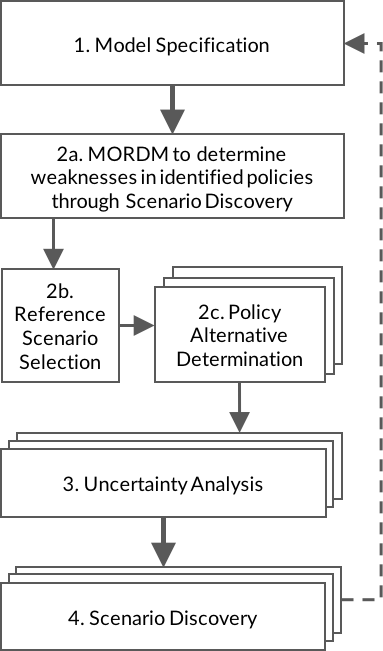
\includegraphics{multi-flow}
        \caption{Multi-Scenario MORDM Process}
        \label{fig:multi-flow}
    \end{figure}
    
    As \cref{fig:multi-flow} demonstrates, the key difference between MORDM and multi-scenario MORDM lies in the search for policy alternatives. The complete and distinct sets of non-dominated policies built from the search involving each reference scenario are all considered throughout the remainder of the method: uncertainty analysis and scenario discovery. 

    Given the proposal to repeat the search for policy alternatives with multiple reference scenarios, the most influential decision in this method will be the selection of reference scenarios. The initial proposal, which is illustrated in \cref{fig:multi-flow} is to use the results of sensitivity analysis performed during the course of MORDM-based analysis as boundaries with which to select the reference scenarios from \citep{Watson2017}. Through this method, \citet{Watson2017} are able to conclude that the use of multiple reference scenarios lead to the discovery of a more diverse set of policy alternatives that perform well under deep uncertainty to consider.
    
    The number of scenarios to select is left to the analyst to determine. By selecting a wide range of scenarios to use as reference points, it is more likely to discover a more diverse set of robust policy options. However, analysis is often limited by computational capabilities and other factors, which means that analysts should search for only a small number of reference scenarios \citep{Eker2018}. There are several criteria that can be considered during the selection process, including internal consistency, diversity of outcome indicators, extremeness, and policy relevance, which may be combined or considered separately depending on goals of the analysis or decision maker preference. \citet{Eker2018} use this information to develop an alternative method of reference scenario selection that is designed for the purpose of finding reference scenarios that, when used in the MOEA search, will lead to more robust solutions, focusing on policy relevance and maximum diversity (where policy relevance is defined as scenarios that lead to outcomes in the lower half of the scenario space and the diversity criterion is based on that which was defined by \citet{Carlsen2016}). \citet{Eker2018} also apply a random approach by selecting a number of scenarios randomly across the uncertainty space, with no consideration for policy relevance or diversity. 

    After applying each mechanism to an intertemporal version of the lake problem (for more details about the lake problem, see \cref{review-problems}), the results using policy relevant reference scenario selection mechanism were shown to lead to a more diverse set of policy alternatives, as well as larger variety of trade-offs in robustness metrics \citep{Eker2018}. The same analysis did not find a signficant difference between the results for the policy relevant scenario selection mechanism and the random mechanism, with both leading to similar increases policy alternative diversity and robust outcome trade-offs \citep{Eker2018}. 
    
    As multi-scenario MORDM is such an new method, there are currently no other applications in literature. Much remains to be learned with respect to the impact of differing scenario selection mechanisms or the effect of using a different number of scenarios on the diversity and robustness of discovered policy alternatives.

    \subsection{Multi-objective robust optimization (MORO)}
    Robust optimization has its roots in mathematical optimization of functions and systems. Traditional optimization algorithms seek the maximum (or minimum) solution(s) generated from a mathematical system and specified input space. In decision making, system optimization commonly refers to determining optimum values for levers which decision makers can use to create the conditions required for a system to reach the targeted outcome. As discussed in \cref{review-robustness} these optima can be unstable and sensitive to even small changes in parameter values. When the system under consideration includes uncertainty, let alone the deep uncertainty present in wicked problems with tipping point characteristics, an optimum that is sensitive to changes in parameter values may easily lead to outcomes that do not hit the desired target. In these cases, a robust solution is desired over an optimum one, which must be accounted for in the optimization process. Early attempts to combine a desire for robustness with a search for optimality occurred in the 1960s \citep{Dorato1966} with the consideration of insensitive optima, and 1970s with the development of an algorithm that seeks the optimum values of levers under worst-case performance settings, given a set of uncertain input parameters \citep{Soyster1973}. It was not until the 1990s, however, that what is now known as robust optimization began to take shape \citep{Sozuer2016}. 
    
    A robust optimization algorithm seeks solutions to a problem that perform reasonably across all potential future states of the world and performs best in worst-case scenarios. Two primary forms of robust optimization have been developed. Deterministic robust optimization uses numerical techniques to determine function optima explicitly. In situations with deep uncertainty, however, it is not possibly to explicitly define all robustness constraints and function variables. In this case, a randomized approach or simulation optimization approach is used \citep{Beyer2007}. Given that wicked problems with tipping point characteristics will always include deep uncertainty, the consideration of robust optimization in this research will focus on simulation optimization.
    
    Robust optima in uncertain models are found through direct evaluation. Robust solutions to the objective function are determined by sampling across the uncertainty space, which can be accomplished in three primary ways \citep{Beyer2007}:
    
    \begin{enumerate}
        \item Monte-Carlo strategies: this involves averaging the objective function values across a sample set of the uncertainty space. Sets of uncertainty values are determined through one of a variety of sampling techniques, including Latin hypercube, Monte-Carlo, and full- and partial-factorial. This method of simulation optimization quickly becomes computationally expensive. 
        \item Meta-model approach: generally used to reduce the computational cost of optimization, a meta-model is carefully constructed to represent the model of interest. Results of optimization using the meta-model are then generalized to estimate optimization results of the original model \citep{Zhou2017}
        \item Optimization using objective function directly: instead of calculating robustness values from the objective function, this method proposes to use the values of the objective function directly to compare policy alternatives \citep{Beyer2007}
    \end{enumerate}
    
    Evolutionary algorithms have been used in combination with Monte-Carlo strategies and noisy optimization to more efficiently obtain robust solutions to a model’s objective function. Evolutionary algorithms are discussed in more detail in \cref{step2-moea}. 

    Previous literature has applied robust optimization techniques as a small step in a larger method of designing policy solutions for a problem characterized by deep uncertainty. \citet{HamaratLoonen2014} uses multi-objective robust optimization as a method of fine-tuning tipping points during adaptive policy making. \citet{Kwakkel2015} makes use of multi-objective robust optimization in the development of Dynamic Adaptive Policy Pathways (DAPP). In this case, robust optimization is used to assess candidate pathways and find the most robust options. Extensions of the MORDM method have approached a multi-objective robust optimization implementation in the search phase by considering more than one reference scenario. In one case, the method continues to determine a policy alternative's dominance through its performance with respect to a single reference scenario at a time \citep{Watson2017}. The closest extension of MORDM is by \citet{Trindade2017}, who, in the context of MORDM, proposes the use of multiple states of the world to calculate robustness and determine whether an alternative is selected during the search phase. However, that approach is specific to the problem under analysis and is not formalized into a prescriptive method for decision support. 
    
    \begin{figure}[ht]
        \centering
        \captionsetup{justification=centering}
        
        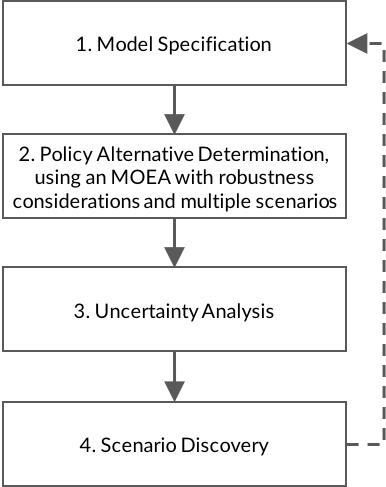
\includegraphics{moro-flow}
        \caption{Multi-Objective Robust Optimization Process}
        \label{fig:moro-flow}
    \end{figure}
    
    This research proposes a multi-objective robust optimization methodology that follows the structure of RDM and can be used as the primary method for analysis to determine the set of robust policy options to a deeply uncertain wicked problem with multiple conflicting objectives. Model specification follows the same XLRM format as was described in \cref{review-rdm}. Robust optimization takes place in the MOEA-based policy alternative determination phase of the method, as illustrated in \cref{fig:moro-flow}. In this stage, policies are compared based on the outcomes of defined robustness metrics, leading to the Pareto optimized set of policies based on robustness. This comparison is compatible with many robustness metrics, depending on the interests of decision makers or the analyst. To enable the calculation of a robustness metric, each policy identified in the MOEA search is evaluated against a set of pre-specified scenarios. The outcomes calculated are then used to determine robustness for each outcome according to the formula of the specified robustness metric. 

    %    A different implementation of the policy alternative determination process is described by \citet{Beh2017}, in which a meta model is used to evaluate robustness, which is determined using a single robustness function. However, by using the model under analysis directly, and by considering each outcome of interest as an independent element of robustness, the search phase is better able to both fully capture the dynamics of the model and consider conflicting objectives, making the robust optimization method proposed in this research a more direct method of incorporating robustness into the search phase of analysis. 
    
    After the search phase is complete, the result is a set of Pareto non-dominated policy solutions that are already considered robust against the set of evaluation scenarios specified for the search. These policies are further tested in uncertainty analysis and scenario discovery to both determine robustness against a significantly larger set of scenarios and find remaining vulnerabilities that can be used to refine the model specification in a new iteration of the analysis. 

    \subsection{The fundamental difference between MORDM, multi-scenario MORDM, and MORO}

    Each of the methods described, MORDM, multi-scenario MORDM, and MORO, are based on the foundations of robust decision support: the RDM method. Though there are many similarities between the three methods, there is one fundamental difference. As highlighted in \cref{fig:diff-flows}, each method takes a different approach to the policy alternative determination phase of the method.
    
    \begin{figure}[ht]
        \centering
        \captionsetup{justification=centering}
        
        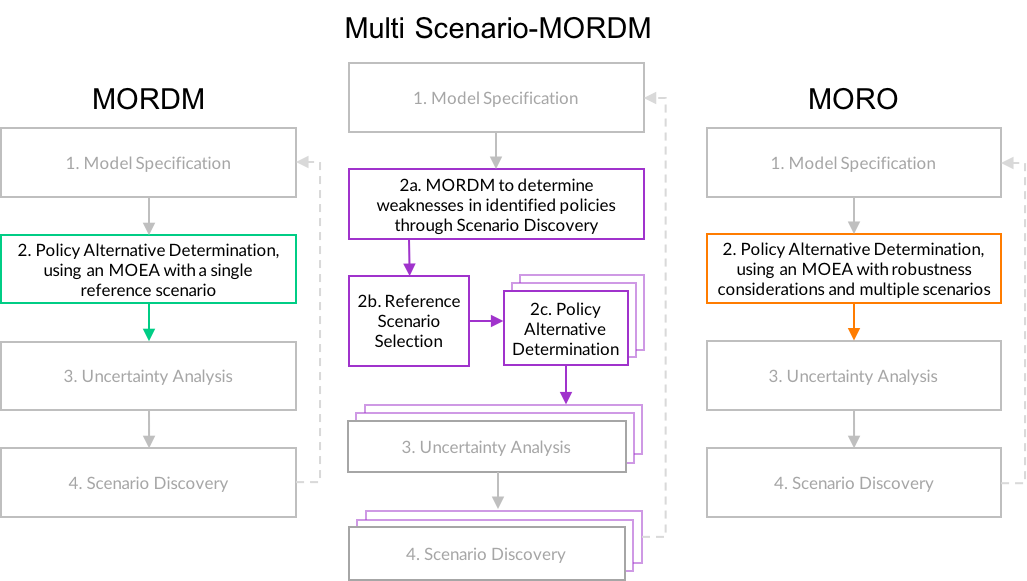
\includegraphics[width=\textwidth]{diff-flows}
        \caption{Comparison of robust decision support method structures}
        \label{fig:diff-flows}
    \end{figure}

    From left to right, the methods increasingly integrate robustness into the policy alternative determination process. MORDM selects policies based on outcomes of interest alone. While multi-scenario MORDM also selects policies based on outcome values, it performs the search using multiple reference scenarios identified from within the vulnerable uncertainty space as determined in scenario discovery of MORDM, thereby introducing small robustness considerations into the search phase. And finally, instead of using outcome values, MORO selects policies by testing each against a pre-defined set of scenarios and using the robustness metric for each outcome, which even more directly brings robustness considerations into the search phase of the method.
    
    As the model specification, uncertainty analysis, and scenario discovery processes are all constant across the three methods, this research will be examining the impact of considering robustness in the policy alternative determination step of an RDM-based method for decision support. 

\section{Problem and Policy Configuration}\label{review-problems}
This section will provide background on the stylized problem used in this study. It will also explore commonly used policy implementation structures, in an effort to select a subset of implementation structures that can be used to test the analytic power of each robust decision support method.

    \subsection{The lake problem}
    In order to compare the methods described in \cref{review-methods}, there must be a usable problem that is representative of the desired behavior. The type of wicked problem under consideration has been identified as including deep uncertainty, a threshold point of no return, where behavior of the system changes dramatically, and the consideration of many decision makers with multiple conflicting criteria. What is known as the shallow lake problem, a common reference problem in policy analysis research, incorporates all of these characteristics. This problem, developed into a policy analysis problem initially by \citep{Carpenter1999}, is a highly stylized decision problem in which a town must decide the amount of pollution to release into a nearby shallow lake over time. As \cref{fig:lake-model} illustrates, this hypothetical problem involves two sources of pollution: anthropogenic pollution generated by the town through industrial and agricultural waste, and natural inflows that are uncontrollable and come from the environment. There is also a natural outflow process based on the capability of the lake to recycle resources that is capable of naturally reducing pollution over time in the lake \citep{Hadka2015}. 

    \begin{figure}[ht]
        \centering
        \captionsetup{justification=centering}
        
        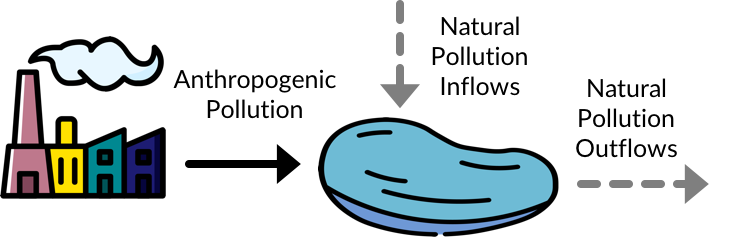
\includegraphics[width=\textwidth]{lake-model}
        \caption{Illustration of pollution flows in lake model}
        \label{fig:lake-model}
    \end{figure}
    
    Through the inflow and outflow processes, the lake's water quality will shift between two states \citep{Carpenter1999}: 

    \begin{itemize}
        \item Oligotrophic equilibrium, with low algae production, high oxygen content, and therefore high fish counts and drinking-water quality
        \item Eutrophic equilibrium, with high levels of algae production and therefore lower fish counts and drinking-water quality. A lake in the eutrophic state reduces the economic benefit of the lake to the nearby town. 
    \end{itemize}

    \begin{figure}[ht]
        \centering
%        \captionsetup{justification=centering}
        
        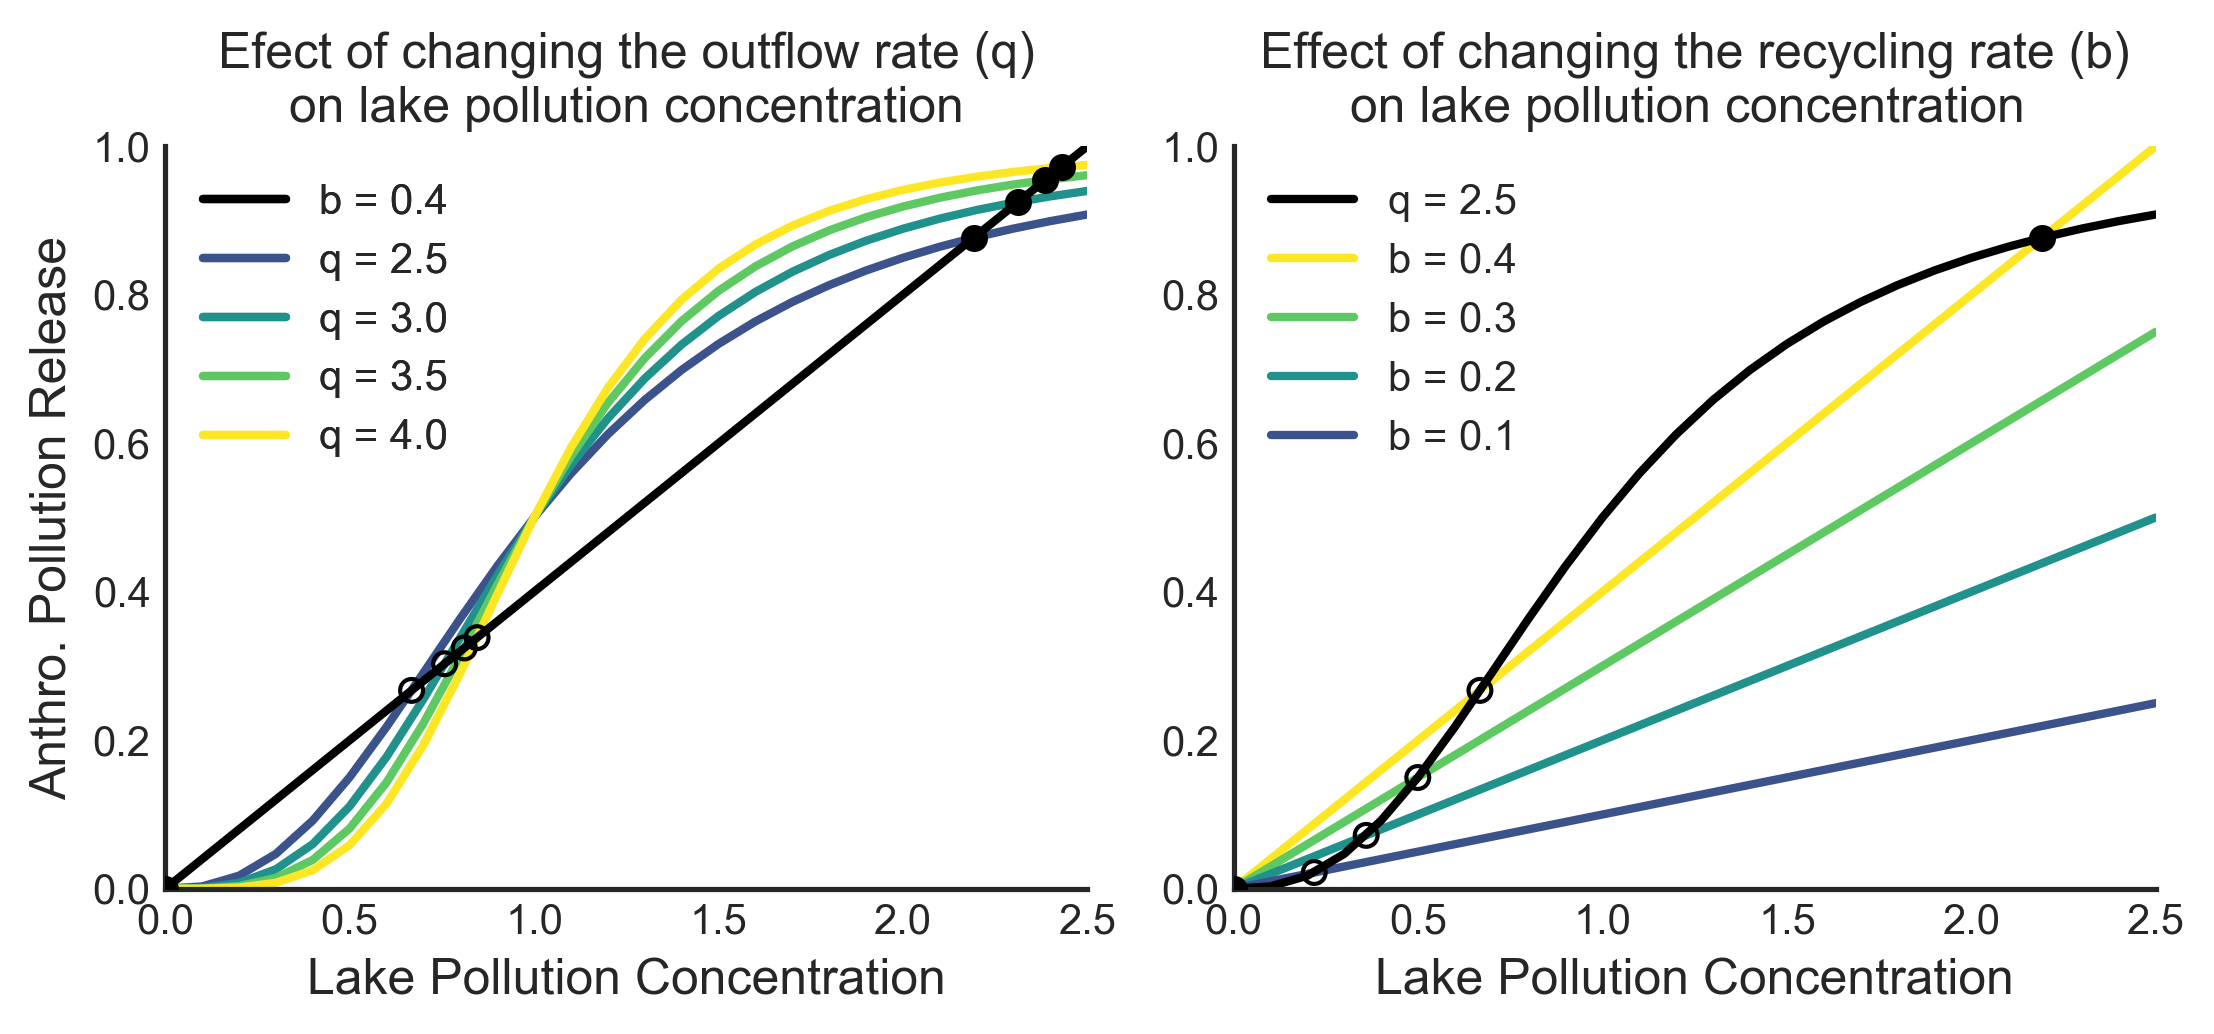
\includegraphics[width=\textwidth]{tippingpoint}
        \caption[Tipping point behavior integrated into the shallow lake problem.]{Illustration of the tipping point behavior present in the lake problem. These plots show the impact of changing the properties that allow the lake to naturally reduce the pollution level on the lake's pollution concentration. Hollow circles represent the unstable equilibrium or tipping point, of the system, while filled circles highlight the stable oligotrophic (at point (0,0) in both plots) and eutrophic equilibrium. Based on a plot found in \citet{Quinn2017}.}
        \label{fig:tippingpoint}
    \end{figure}
    
    Pollution levels are determined through \cref{eq:pollution}, where \textit{X} represents the concentration of pollution in the lake, \textit{a} is the anthropogenic pollution input for the time period, \textit{Y} refers to the natural inflows of pollution, \textit{q} indicates the recycling rate at which pollution is removed from the lake through recycling by the lake's sediment, and \textit{b} refers to the loss of pollution from the lake through natural outflows. The exact specifications for each of the parameters are based on the lake model developed by \citet{Quinn2017}. 

    \begin{equation}\label{eq:pollution}
        X_{t+1} = X_{t} + a_{t} + Y_{t} + \frac{X_{t}^{q}}{1+X_{t}^{q}} - bX_{t}
    \end{equation}

    Because the lake problem is designed to include tipping point behavior, the transition between the two states may be rapid and result from even a small change in inflow levels. When the critical threshold of pollution concentration is surpassed, the trend transitions toward eutrophic equilibrium, making impossible to return to a healthier oligotrophic equilibrium without active human intervention to reduce the pollution level in the lake \citep{Quinn2017}. This is visualized in \cref{fig:tippingpoint}. Both panels indicate that the more pollution a lake is able to remove naturally, the higher the lake's tipping point is, making it easier to avoid the point of no return and a eutrophic equilibrium. 
    
    The characteristics of the lake problem also allow it to incorporate competing desires between maximizing a town's economic productivity by maximizing anthropogenic pollution release, and minimizing negative impacts on the lake's water quality to ensure a healthy environment for fishing, leisure, and other activities \citep{Ward2015}. 
    
    There are several benefits from using this stylized problem over a case study based on specific real-world properties. First, the behavior described by the lake problem can be considered similar to the behavior of many other real-world issues that include a balance between generation of sources that can negatively impact a system with the loss of benefits when that system is negatively impacted. This dynamic is especially common in environmental problems like climate change and other pollution-related issues \citep{Carpenter1999}. Second, by using a relatively straightforward model, it is easy to catalog assumptions and omissions, which enables more rigor when assessing the effectiveness of different robust decision support methods. And finally, by using a stylized problem that has been used in research before, there is a stronger foundation for comparison and validity of results with respect to that problem and its characteristics. 

    \subsubsection{Sources of uncertainty}
    The lake problem that is used for this research includes five sources of uncertainty. As indicated in \cref{eq:pollution}, $b$ and $q$ indicate the ability of the lake to remove pollution through natural processes. Two additional sources of uncertainty relate to the natural inflows of pollution to the lake from the environment, where the inflow, $Y$ is represented as a function of $\mu$, the mean of natural inflows for the lake, and $\sigma^{2}$, the standard deviation of natural inflows \citep{Quinn2017}. The remaining source of uncertainty $\delta$, represents the future discount rate of utility. 

    \subsubsection{Objectives}
    Along with the five sources of uncertainty, the lake problem identifies four conflicting objectives: maximum pollution level, utility of the release policy to the town, reliability of the policy, and policy inertia. The multi-objective form of this problem was introduced by \citet{Singh2015} and further developed by \citet{Ward2015}, with the goal of introducing objectives that exemplify the conflicts that occur with a diverse group of decision makers and a problem characterized by deep uncertainty.
    
    \textbf{Maximum Pollution (minimize)}: Some decision makers are seeking to ensure that the maximum pollution level reached in the lake is kept to as low a value as possible. This objective represents the perspective of environmental regulators who strive to maintain the health of the lake \citep{Singh2015}.
    
    \textbf{Reliability (maximize)}: Representing the interest of key decision makers who are especially concerned with keeping the lake in an oligotrophic state, because they depend on it for income, recreation, or some other purpose. Reliability captures desire of decision makers to keep the lake below the critical pollution threshold. At the same time, in contrast with the maximum pollution objective which strives to strictly minimize pollution, a policy that has high reliability is also accepting of a small amount of pollution, as long as it remains under that critical threshold \citep{Singh2015}.

    \textbf{Utility (maximize)}: To contrast the objectives that relate the goals common among environmental regulators, utility represents the interests of the town's agriculture and industry, with the goal being to maximize the utility of a policy for those decision makers. This objective naturally conflicts with the objective of minimizing the pollution level in the lake, providing a valuable dynamic for robust decision support analysis \citep{Ward2015}. 
    
    \textbf{Inertia (maximize)}: Capturing the interests of the lake manager, this objective refers to the stability of the pollution release amount over time. As dramatic changes in pollution will require large infrastructure investments, it is in the lake manager's interest to maintain a steady level of pollution release over time \citep{Quinn2017}. 

    \subsection{Policy implementation structure} \label{review-structure}
    Given a deeply uncertain problem with several sources of uncertainty and multiple conflicting objectives, the next step of analysis is to establish a strategy or policy that helps decision makers reach their objectives. There are two approaches to policy development, each of which are fundamentally different and have varying internal characteristics \citep{Maier2016}.
    
    \textbf{Static}: A fixed strategy that is fixed and is not adjusted despite changes in the system. A static solution can be one decision that is being made at the start of the time horizon being considered. Alternatively, a static policy can consist of multiple decisions that are executed at predetermined points in the time horizon.
    
    \textbf{Adaptive}: A flexible strategy that responds to changing conditions or increased knowledge about the current or future state of the world. Adaptive policies can be implemented in different ways: 
    \begin{itemize}
        \item A static adaptive approach, in which there is a static policy in place that remains fixed and is supported by contingency actions to help keep the system in a good state. 
        \item A dynamic approach to adaptation, in which the available set of policy options itself changes based on changing conditions or new knowledge about the future state of the world. 
    \end{itemize}

    The comparisons made in this research will consider three policy structure alternatives, based on those identified above.

    \textbf{Intertemporal}: Also known as open-loop control, this variation of the lake problem has been used in research several times and involves a series of pre-determined static decisions made every time-step \citep{Hadka2015,Quinn2017,Singh2015,Ward2015}. This option represents a strictly static approach to solving the lake problem. 

    \textbf{Direct Policy Search}: Representing the other extreme in policy structure, direct policy search (DPS), or closed-loop control. Instead of building a policy that defines anthropogenic pollution release levels, the DPS structure involves optimizing a set of parameters that form a state-aware pollution release rule. This control rule is used to update the level of pollution released at every time-step, giving this policy structure the ability to quickly respond to changes in system conditions. The DPS structure has also been used as a part of the lake problem in research before \citep{Quinn2017}. 
    
    \textbf{Planned Adaptive DPS}: Given that both the intertemporal and DPS policy structures adapt the pollution release every time period, they do not necessarily represent real-world decision strategy, where it takes time to implement changes. Therefore, this research is proposing a third policy structure that follows the same fundamental structure of the DPS policy, but updates the level of pollution that is released every time step every N time steps (instead of every time step, as in traditional DPS), where N is a number set by the decision makers or policy analysts. 
